%%%%%%%%%%%%%%%%%%%%%%%%%%%%%%%%%%%%%%%%%%%%%%%%%%%%%%%%%%%%
%%% LIVECOMS ARTICLE TEMPLATE FOR BEST PRACTICES GUIDE
%%% ADAPTED FROM ELIFE ARTICLE TEMPLATE (8/10/2017)
%%%%%%%%%%%%%%%%%%%%%%%%%%%%%%%%%%%%%%%%%%%%%%%%%%%%%%%%%%%%
%%% PREAMBLE
\documentclass[9pt,software]{livecoms}
% Use the 'onehalfspacing' option for 1.5 line spacing
% Use the 'doublespacing' option for 2.0 line spacing
% Use the 'lineno' option for adding line numbers.
% Use the "ASAPversion' option following article acceptance to add the DOI and relevant dates to the document footer.
% Use the 'pubversion' option for adding the citation and publication information to the document footer, when the LiveCoMS issue is finalized.
% The 'bestpractices' option for indicates that this is a best practices guide.
% Omit the bestpractices option to remove the marking as a LiveCoMS paper.
% Please note that these options may affect formatting.

\usepackage{lipsum} % Required to insert dummy text
\usepackage[version=4]{mhchem}
\usepackage{siunitx}
\DeclareSIUnit\Molar{M}
\usepackage[italic]{mathastext}
\graphicspath{{pictures/}}

%%%%%%%%%%%%%%%%%%%%%%%%%%%%%%%%%%%%%%%%%%%%%%%%%%%%%%%%%%%%
%%% IMPORTANT USER CONFIGURATION
%%%%%%%%%%%%%%%%%%%%%%%%%%%%%%%%%%%%%%%%%%%%%%%%%%%%%%%%%%%%

\newcommand{\versionnumber}{1.0}  % you should update the minor version number in preprints and major version number of submissions.
\newcommand{\githubrepository}{\url{https://github.com/thehamop1/AdvSoftwareEngineeringProject}}  %this should be the main github repository for this article

%%%%%%%%%%%%%%%%%%%%%%%%%%%%%%%%%%%%%%%%%%%%%%%%%%%%%%%%%%%%
%%% ARTICLE SETUP
%%%%%%%%%%%%%%%%%%%%%%%%%%%%%%%%%%%%%%%%%%%%%%%%%%%%%%%%%%%%
\title{Designing a scalable Conversational Interfaces}

\author[1\authfn{3}]{Cristian Gutierrez}
\author[1\authfn{3}]{Darshi Kasondra}
\author[1\authfn{3}]{Archana Ravi}
\author[1\authfn{3}]{Mounica Dingari}
\affil[1]{California State University of Northridge}

\corr{cristian.gutierrez.56@my.csun.edu}{CG}  % Correspondence emails.  FMS and FS are the appropriate authors initials.

\presentadd[\authfn{3}]{Department of Engineering and Computer Science, California State University of Northridge, United States of America}

\blurb{Additional work related to this paper can be fournd at \githubrepository;}

%%%%%%%%%%%%%%%%%%%%%%%%%%%%%%%%%%%%%%%%%%%%%%%%%%%%%%%%%%%%
%%% PUBLICATION INFORMATION
%%% Fill out these parameters when available
%%% These are used when the "pubversion" option is invoked
%%%%%%%%%%%%%%%%%%%%%%%%%%%%%%%%%%%%%%%%%%%%%%%%%%%%%%%%%%%%
\pubDOI{10.XXXX/YYYYYYY}
\pubvolume{<volume>}
\pubissue{<issue>}
\pubyear{<year>}
\articlenum{<number>}
\datereceived{Day Month Year}
\dateaccepted{Day Month Year}

%%%%%%%%%%%%%%%%%%%%%%%%%%%%%%%%%%%%%%%%%%%%%%%%%%%%%%%%%%%%
%%% ARTICLE START
%%%%%%%%%%%%%%%%%%%%%%%%%%%%%%%%%%%%%%%%%%%%%%%%%%%%%%%%%%%%

\begin{document}

\begin{frontmatter}
\maketitle

\begin{abstract}
The way we use interact with systems is contantly evolving with new advances in technology. As buisness continue to need flexible user
interfaces many of them are implementing conversatinal interfaces in order to fufill customer needs without having to require users
to learn how to use an entirely seperate application in order to make transactions. Modern conversatinal interfaces are fairly powerful 
with recent adavancements in natural language processing, integration with mobile asistants, and flexible frameworks. In this paper we 
provide background to some of the concepts of conversatinal interfaces, examing the current state of commercially available
solutions, and provide a reference architecture for implementing a system centered around a conversatinal interface.
\end{abstract}

\end{frontmatter}

\section{Introduction}

\subsection{Previous Work, Methods, Procedures}
There is a growing need for approchable user interfaces as more interactions become digital. For example banking, transactions, and flights
are all largely growing to be digital. In order to easily accessed and usable for all types of users conversatinal interfaces are the most 
ideal due to their low learning curve. If a user can use their native language in order to complete actions on any given system the need for
24/7 support or complex user interfaces become obsolete. This allows buisness to keep user satisfaction high while keeping costs low. Additionally
it provides several benefits to users as they are able to access data from large databases easily, complete transactions even if their not so tech savy,
have multilingual support, and have 24/7 support.
\subsection{Previous Work, Methods, Procedures}
The development and interest of conversatinal interfaces was has been a subject of interest since the 1970's. Early examples of these
early chatbots include ELIZA, ALICE, and PARRY. Many of these early chatbots worked with the use of simple pattern matching. This simple 
regular expression based matching was combined with a tree design for controlling the flow of conversations. One of the major drawbacks of 
this naive form of design was the frequent matching of user utterances with conversation points that happened further up the tree. This 
would often lead to looping conversations. Researchers at the time had to develop markup based langugues such as AIML in order to develop 
expert systems. These large complex forms of nested databases had to be constantly maintined in order to add new features to these chatbots. 
With the modern development of machine learning algorithms in order to parse and extract meaning from user utterances. Many commercial solutions
for developing conversatinal interfaces are now widely available and come with many integrations for various platforms.
\subsection{Background}
There are some basic concepts that are universal to most conversatinal interface platforms. The first is the user utterance which can either come in 
the form of a text entry or speech with the use of a microphone. Additional signal processing is required to transcribe the audio signals into text. 
This text is usually normalized where all text has its puntuation removed and all letters are moved into the same letter case. Next depending on the 
platform various machine learning algorithms are used in order to extract certain key tokens from the string. The most intent which is the objective
of the user. For example the utterance "What is the weather in Los Angeles" would have the intenet of weather. This is a topic that the application
would have to be designed to respond to. Next would be entities which are certain tokens the application will use to complete requests once an intenet
has been deduced.

\section{Implementation Guide}
\subsection{Use Cases}
The following implementation guide was designed with the assumption that it would be used in a buisness context such as 
e-commerce site, resturant, or customer support. Additionally little sensitive information would be transmitted between the 
conversatinal interface and the service could be an addition to existing buisness infrastructure. Additionally this 
Implementation guide is more suitable for small to medium sized buisness who are looking to provide the user with 
the ability to retrieve basic data and transactions.

An example use case for this reference architecture would be a small chain of resturants. In this scenario a customer may
want to make reservations for instance while the resturant is closed. In this scenario integrating a conversatinal interface 
on the buisnesses website and mobile assistant would provide the user with the ability to create or cancel reservations while 
the buisness is currently closed. Even customers with little knowledge of how to browse the internet or create reservations online
would be able to interact with their mobile asistants in order to interact with the system.  

\subsection{Technical Stack}
For this particular implementation guide a stack such as ReactJs, SQL, nodejs, dialogflow, and Google Assistant/Siri would be used. NodeJS would
be used on the lambda functions and buisness enterprise. Any in buisness databases would be created with an SQL flavor and an ORM such as 
knex.js would be used to store various information. If a buisness did not have an existing website it would be created in ReactJS, alternatively 
if an existing website was already available a simple iframe based solution could be used from the existing dialogflow API integrations.

As stated before any interaction needed with existing buisness infrastructure could be handled with lambda funcitons. The existing language most 
supported by the Dialogflow API is NodeJS. It is extermly cost effective and easy to integrate using Google Cloud Functions. In order to fully take
advantage of deploying to various platforms different buisness logic needs to created to interact with various front-ends. The Dialogflow API allows
you to create specific reponses based on the clients platform in order not to overwhelm the client with long responses or provide more relevant information
to the user.  

An added benefit to using lambda functions is that all of the heavy machine learning processing is carried out on the Dialogflow API side so no heavy
processing is required within the runtime of the lambda itself. This allows the call from the client to be quickly parsed via a RESTful API call and 
intenets, entities, and context can already be deduced ahead of time. By allowing the buisness logic to be compeltley free of all machine learning it allows
the particular buisness implemnting the system save money on renting a fully dedicated server to run the machine learning algorithm. Keep in mind that although
the use of lambda functions reduces cost there is an additonal cost required for every call to the Dialogflow service. Additionally the version of the DialogFlow API 
used also factors into cost. If the complexity of the conversations are relativley simple version 2 of the API can be used to increase savings on this implementation.

The Dialogflow dashboard would need to be trained using a set of sample training data. Most of the internal machine learning algorithms are abstracted on this platform. 
What this means for the buisness trying to develop their platform with this tool is that the develop who they chose to hire doesnt need an extensive background in machine
learning in order to get things working in the first place. In addition to this sample training data simple regular expressions would be given to the DialogFlow agent in order
to fall back on when confidence scores get too low. 

Lastly in terms of getting a voice enabled conversatinal interface for this systmem would require the use of the newer DialogFlow V3 API or the use of a deprecated 
API in order to interface wtih the older DialogFlow version 2. Although this option is available using the newer nodejs package it is highly discouraged as this part
of the library is no longer receiveing updates. Additionally in order to connect this service to iOS an additionial layer of buisness logic has to be placed between the 
dialogflow API calls and the Siri front-end. The buisness should consider the development cost required in order to keep iOS integration supported versus how 
benefical it is from a buisness stand-point to keep it supported. 

\subsection{Cost Benefit Analysis}
In order to understand the on-going cost of having lambda function costs and DialogFlow API calls the following charts should be considered when 
considering the benefit of adding a converstaional interface to an e-commerce site. 

\begin{figure}
  \caption{DialogFlow Version 2}
  \centering
    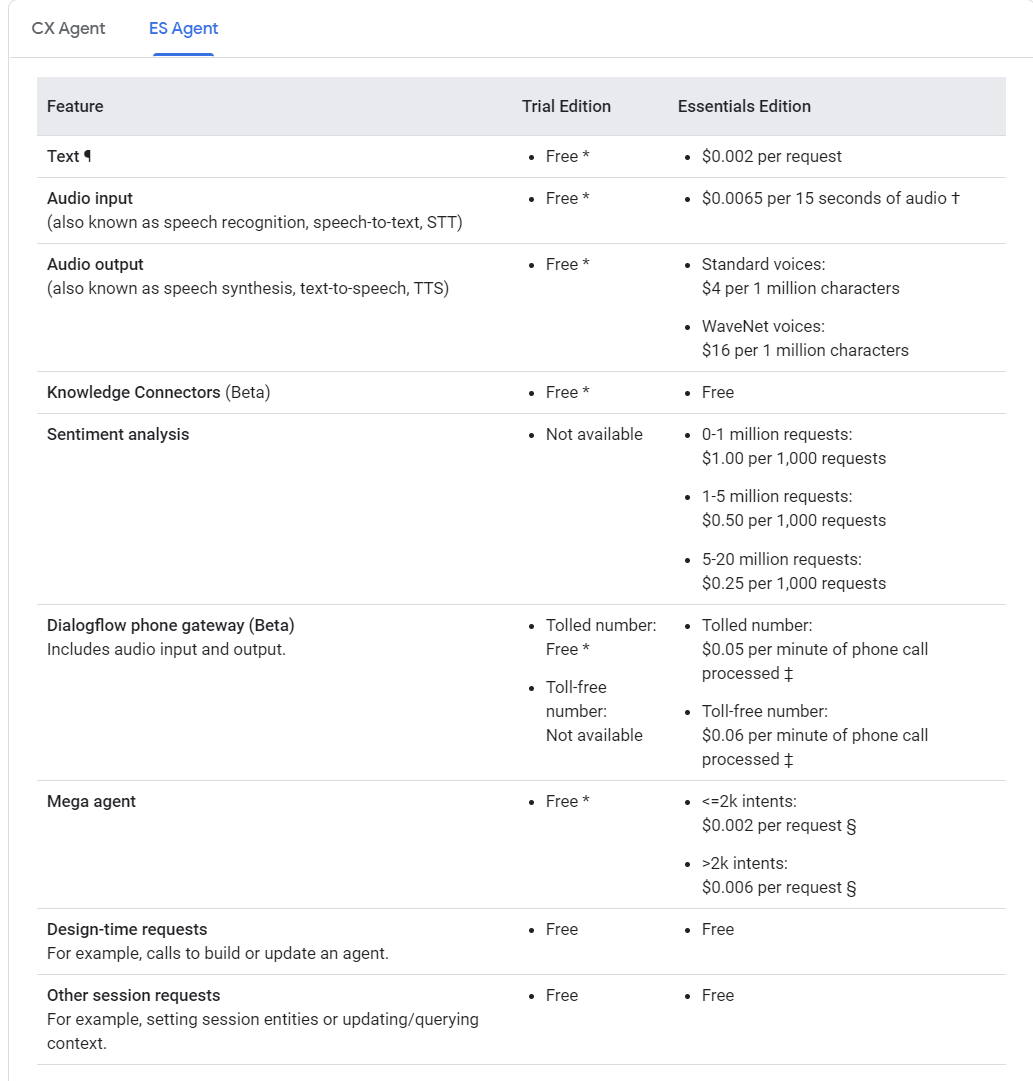
\includegraphics[width=0.5\textwidth]{ESAgent.PNG}
\end{figure}

\begin{figure}
  \caption{DialogFlow Version 3}
  \centering
    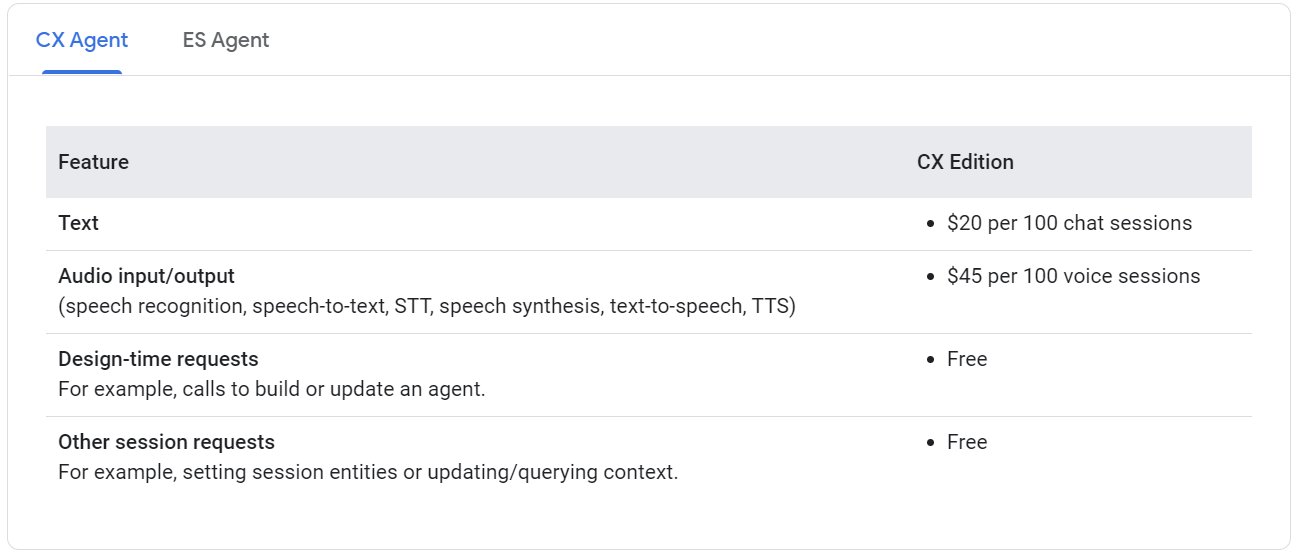
\includegraphics[width=0.5\textwidth]{CX_Agent.PNG}
\end{figure}

As seen above the cost of supporting the converstational interface API version 3 is far different that supporting version 2. If the buisness needs don't demand strict requirements 
that users will be generating complex utterances then version 2 of the API should be considered. If integration with google assistant and siri is an important feature then it's recommended
that Google Actions API be used (DialogFlow v3). Additionally the price of Google Cloud Function calls should also be considered. This service has a much lower cost especially if compute times
are kept low. See Figure 3.

\begin{figure}
  \caption{Google Cloud Function Pricing}
  \centering
    % 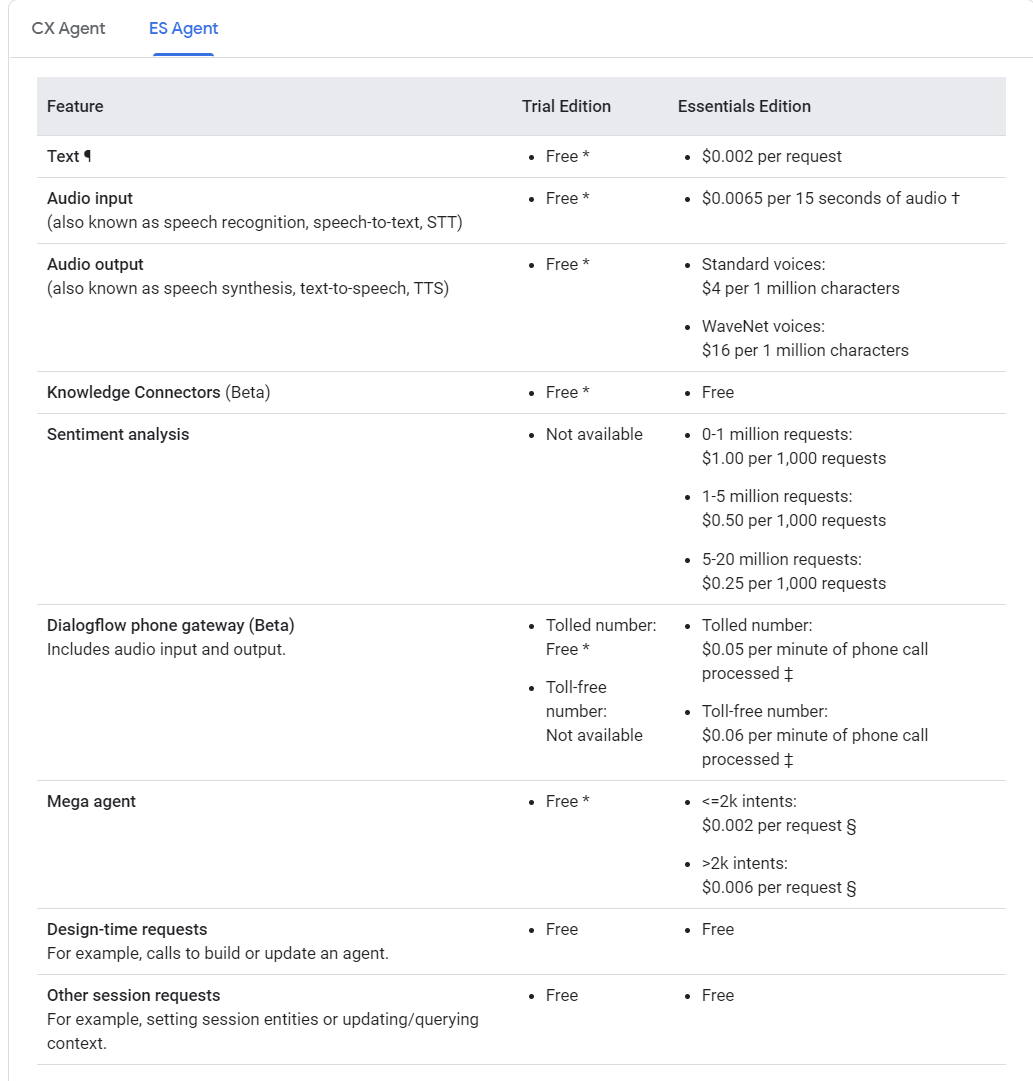
\includegraphics[width=0.5\textwidth]{ESAgent.PNG}
\end{figure}

\section{Development Plan}
\subsection{Configuration Management}
Within the Google Cloud Function dashboard a repository should be connected as the main source code for the lambda functions that will be servicing DialogFlow requests. This repository should be configured
with either the Github Flow or Git Flow configuration style. That being said in order to prevent disastrous situation such as a novice developer pushing to the deployment branch Continous Integration should
be implemented in order to verify that the deployed source code will work in production. Google Cloud can be configured in such a way most of the source conrol lives in Github or Bitbucket where the git server
can be configured to interact with Jenkins CI or Travis CI. Upon certain actions such as merging to the master the repository can automatically launch the newest source code
to the active lambdas.

\subsection{Developer Environment}



% \section{Methodology}

% Here (and in other sections if needed) you would describe how you compared the software in question, with subsections as needed.
% Perhaps you may also need to comment here on why you did not include certain pieces of software or how these might be included in the future.

% \subsection{Physical systems and properties}

% What did you calculate, on what systems? Why did you make that choice?

% \subsection{Methodology for comparison}
% How did you compute what you're comparing?
% What software versions did you use?
% How would the software be accessed?


% \subsubsection{Method selection}
% How did you select which protocols to use? How are you certain these are representative? Would a naive user get similar performance?

% \subsubsection{Supporting files}
% Are there run scripts or files others would need to reproduce your work? Are these provided in your GitHub repo, or how would they be accessed?
% How exactly would someone reproduce/extend this work?

% \subsubsection{Error analysis}
% You may wish to devote particular attention to error analysis.


% \section{Results}

% You would give results.


% \section{Discussion and conclusions}

% You may perhaps wish to revisit the issue of what performance a naive user might expect, here.



% \section{Author Contributions}
%%%%%%%%%%%%%%%%
% This section mustt describe the actual contributions of
% author. Since this is an electronic-only journal, there is
% no length limit when you describe the authors' contributions,
% so we recommend describing what they actually did rather than
% simply categorizing them in a small number of
% predefined roles as might be done in other journals.
%
% See the policies ``Policies on Authorship'' section of https://livecoms.github.io
% for more information on deciding on authorship and author order.
%%%%%%%%%%%%%%%%

% (Explain the contributions of the different authors here)

% We suggest you preserve this comment:
% For a more detailed description of author contributions,
% see the GitHub issue tracking and changelog at \githubrepository.

% \section{Other Contributions}
%%%%%%%%%%%%%%%
% You should include all people who have filed issues that were
% accepted into the paper, or that upon discussion altered what was in the paper.
% Multiple significant contributions might mean that the contributor
% should be moved to authorship at the discretion of the a
%
% See the policies ``Policies on Authorship'' section of https://livecoms.github.io for
% more information on deciding on authorship and author order.
%%%%%%%%%%%%%%%

% (Explain the contributions of any non-author contributors here)
% We suggest you preserve this comment:
% For a more detailed description of contributions from the community and others, see the GitHub issue tracking and changelog at \githubrepository.

% \section{Potentially Conflicting Interests}
%%%%%%%
%Declare any potentially competing interests, financial or otherwise
%%%%%%%

% Declare any potentially conflicting interests here, whether or not they pose an actual conflict in your view.

% \section{Funding Information}
%%%%%%%
% Authors should acknowledge funding sources here. Reference specific grants.
%%%%%%%
% FMS acknowledges the support of NSF grant CHE-1111111.

\bibliography{livecomsm-template-softwareanalyses}

%%%%%%%%%%%%%%%%%%%%%%%%%%%%%%%%%%%%%%%%%%%%%%%%%%%%%%%%%%%%
%%% APPENDICES
%%%%%%%%%%%%%%%%%%%%%%%%%%%%%%%%%%%%%%%%%%%%%%%%%%%%%%%%%%%%

%\appendix


\end{document}
